%package list
\documentclass{article}
\usepackage[top=3cm, bottom=3cm, outer=3cm, inner=3cm]{geometry}
\usepackage{graphicx}
\usepackage{url}
\usepackage{multirow}
%\usepackage{cite}
\usepackage{hyperref}
\usepackage{array}
\usepackage{multicol}
\newcolumntype{x}[1]{>{\centering\arraybackslash\hspace{0pt}}p{#1}}
\usepackage{natbib}
\usepackage{pdfpages}
\usepackage{multirow}
\usepackage{float}
\usepackage[normalem]{ulem}
\useunder{\uline}{\ul}{}




%%%%%%%%%%%%%%%%%%%%%%%%%%%%%%%%%%%%%%%%%%%%%%%%%%%%%%%%%%%%%%%%%%%%%%%%%%%%
%%%%%%%%%%%%%%%%%%%%%%%%%%%%%%%%%%%%%%%%%%%%%%%%%%%%%%%%%%%%%%%%%%%%%%%%%%%%
\newcommand{\csemail}{vmachacaa@unsa.edu.pe}
\newcommand{\csdocente}{Vicente Machaca Arceda}
\newcommand{\cscurso}{Algoritmos y Estructura de Datos}
\newcommand{\csuniversidad}{Universidad Nacional de San Agustín}
\newcommand{\csescuela}{Maestría en Ciencia de la Computación}
\newcommand{\cspracnr}{03}
\newcommand{\cstema}{--}
%%%%%%%%%%%%%%%%%%%%%%%%%%%%%%%%%%%%%%%%%%%%%%%%%%%%%%%%%%%%%%%%%%%%%%%%%%%%
%%%%%%%%%%%%%%%%%%%%%%%%%%%%%%%%%%%%%%%%%%%%%%%%%%%%%%%%%%%%%%%%%%%%%%%%%%%%


\usepackage[english,spanish]{babel}
\usepackage[utf8]{inputenc}
\AtBeginDocument{\selectlanguage{spanish}}
\renewcommand{\figurename}{Figura}
\renewcommand{\refname}{Referencias}
\renewcommand{\tablename}{Tabla} %esto no funciona cuando se usa babel
\AtBeginDocument{%
	\renewcommand\tablename{Tabla}
}

\usepackage{fancyhdr}
\pagestyle{fancy}
\fancyhf{}
\setlength{\headheight}{30pt}
\renewcommand{\headrulewidth}{1pt}
\renewcommand{\footrulewidth}{1pt}
\fancyhead[L]{\raisebox{-0.2\height}{
\includegraphics[width=3cm]{Img/logo_unsa.jpg}}}
\fancyhead[C]{}
\fancyhead[R]{\fontsize{7}{7}\selectfont	\csuniversidad \\ \csescuela \\ \textbf{\cscurso} }
\fancyfoot[L]{MSc. Vicente Machaca}
\fancyfoot[C]{\cscurso}
\fancyfoot[R]{Página \thepage}







\begin{document}
	
	\vspace*{10px}
	
	\begin{center}	
		\fontsize{17}{17} \textbf{ Práctica \cspracnr}
	\end{center}
	%\centerline{\textbf{\underline{\Large Título: Informe de revisión del estado del arte}}}
	%\vspace*{0.5cm}
	

	\begin{table}[h]
		\begin{tabular}{|x{4.7cm}|x{4.8cm}|x{4.8cm}|}
			\hline 
			\textbf{DOCENTE} & \textbf{CARRERA}  & \textbf{CURSO}   \\
			\hline 
			\csdocente & \csescuela & \cscurso    \\
			\hline 
		\end{tabular}
	\end{table}	
	
	
	\begin{table}[h]
		\begin{tabular}{|x{4.7cm}|x{4.8cm}|x{4.8cm}|}
			\hline 
			\textbf{PRÁCTICA} & \textbf{TEMA}  & \textbf{DURACIÓN}   \\
			\hline 
			\cspracnr & Algoritmos de ordenamiento  & 3 horas   \\
			\hline 
		\end{tabular}
	\end{table}
	
	
	\section{Datos de los estudiantes}
	Grupo: N° 8
	\begin{itemize}
		\item Integrantes: 
		\begin{itemize}
			\item Esai Josue Huaman Meza
			\item Alan Jerry Reyes Robles
			\item Jorge Luis Zegarra Guardamino
			\item Nestor Giraldo Calcinas Huaranga
		\end{itemize}		
	\end{itemize}
	
	
	
	
	
	
	\section{Introducción}
	
	Para esta Práctica, se implemetará la estructura multidimensional QuaqTree.

    Para esto se usará los códigos dados por el docente en la práctica y así mismo se terminarán de colocar algunos algoritmos faltantes. Luego de ello se modificará y se mostrará en in index.html los resultados.

    Para todo ello, el lenaguaje de programamción a usar será Java Script.
	
	
	\section{Estructuras de Datos Multidimensional}\label{sec:ejercicios}
	\begin{enumerate}
		\item \textbf{Estructura de datos Quadtree}
		
			La estructura de Datos Quadtree, o árbol cuaternario, se utiliza para describir clases de estructuras de datos jerárquicas cuya propiedad común es que están basados en el principio de descomposición recursiva del espacio.

La Estructura Quadtree se describe de la siguiente manera: 

\begin{itemize}
   \item En un QuadTree de puntos, el centro de una subdivisión está siempre en un punto.
   \item Al insertar un nuevo elemento, el espacio queda divido en cuatro cuadrantes.
   \item Al repetir el proceso anterior, el cuadrante se divide de nuevo en cuatro cuadrantes, y así sucesivamente.
   \item El estructura Quadtree se usa para describir una clase de estructuras jerárquicas cuya propiedad en común es el principio de recursividad de descomposición del espacio.
\end{itemize}	

\begin{figure}[H]
\centering
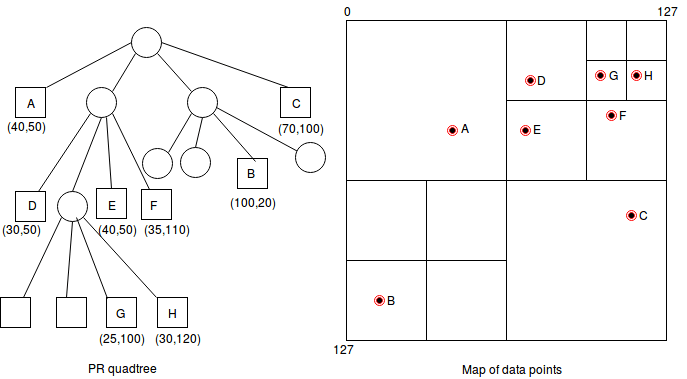
\includegraphics[width=0.9\textwidth]{Img/Quadtree.jpg}
\caption{Estructura QuadTree}
\end{figure}

\end{enumerate}

\section{Implementación}

  Se desarrolló la estructura QuadTree implementando los cambios solicitados en la práctica, los cuales se pueden encontrar en el siguiente repositorio Github \href{https://github.com/josuemzx/QuadTree_js}{Estructuras Quadtree}, y se obtienen las siguientes imágenes.


\section{Resultados}

    \begin{enumerate}
    
        \item \textbf{Estructura QuadTree}

\begin{itemize}
   \item Crear un archivo main.html
\end{itemize}

\begin{figure}[H]
\centering
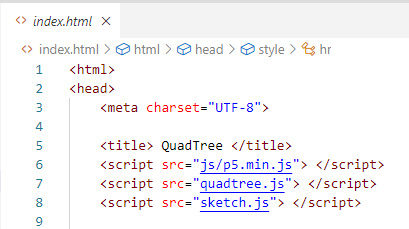
\includegraphics[width=0.7\textwidth]{Img/index.png}
\caption{Archivo main.html}
\end{figure}

\begin{itemize}
   \item Crear un archivo quadtree.js
\end{itemize}

\begin{figure}[H]
\centering
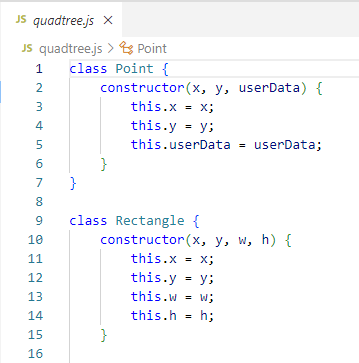
\includegraphics[width=0.6\textwidth]{Img/quadtree.png}
\caption{Archivo quadtree.js}
\end{figure}

\begin{itemize}
   \item Crear un archivo sketch.js
\end{itemize}

\begin{figure}[H]
\centering
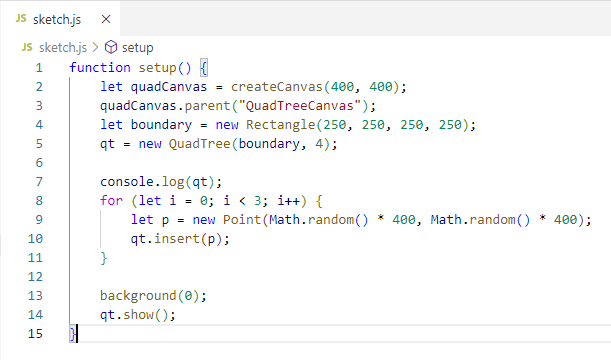
\includegraphics[width=0.9\textwidth]{Img/sketch.png}
\caption{Archivo sketch.js}
\end{figure}

\begin{itemize}
   \item Resultado hasta el momento, se visualiza el QuadTree de tamaño 400 x 400 con 3 puntos.
\end{itemize}

\begin{figure}[H]
\centering
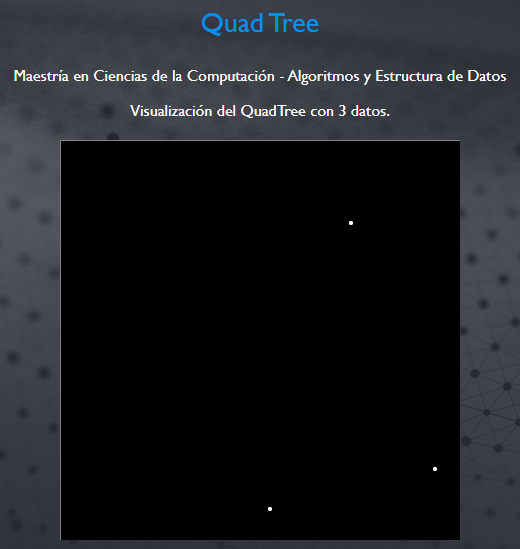
\includegraphics[width=0.6\textwidth]{Img/tres puntos_quadtree.png}
\caption{Visualización Quadtree con 3 puntos}
\end{figure}

\begin{itemize}
   \item Visualización de la Consola del Navegador y ubicar los 3 puntos anteriores.
\end{itemize}

\begin{figure}[H]
\centering
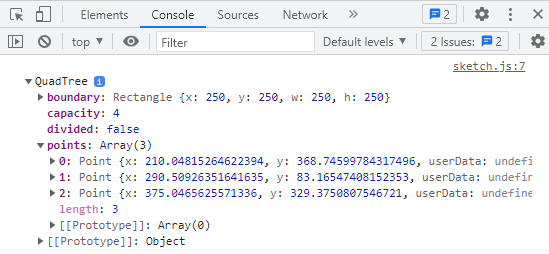
\includegraphics[width=1\textwidth]{Img/consola_web_quadtree.png}
\caption{Visualización de la Consola del Navegador}
\end{figure}

\begin{itemize}
   \item Editar el archivo sketch.js para que se pueda insertar puntos utilizando el mouse.
\end{itemize}

\begin{figure}[H]
\centering
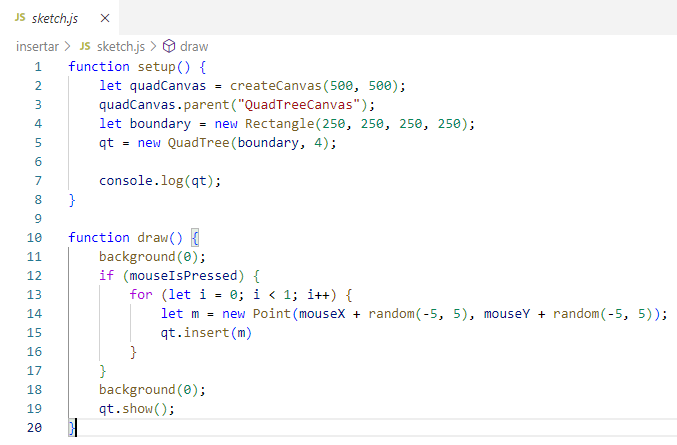
\includegraphics[width=0.9\textwidth]{Img/sketch_insert.png}
\caption{Algoritmo actualizado en el archivo sketch.js}
\end{figure}

\begin{itemize}
   \item Resultado hasta el momento, se insertan puntos utilizando el mouse.
\end{itemize}

\begin{figure}[H]
\centering
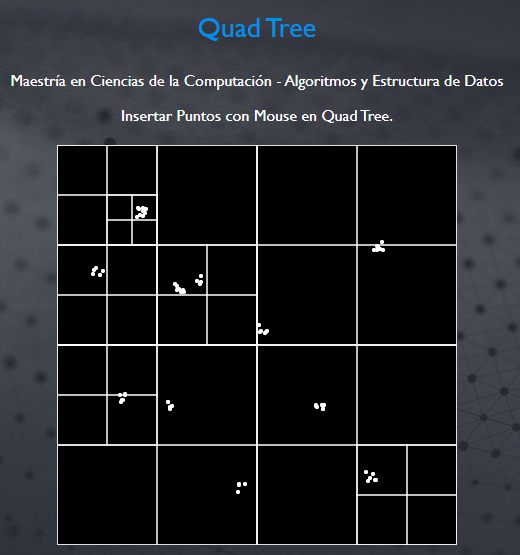
\includegraphics[width=0.5\textwidth]{Img/insertar puntos_quadtree.png}
\caption{Visualización Quadtree con inserción de puntos}
\end{figure}

\begin{itemize}
   \item Editar el archivo quadtree.js y completar la función query.
\end{itemize}

\begin{figure}[H]
\centering
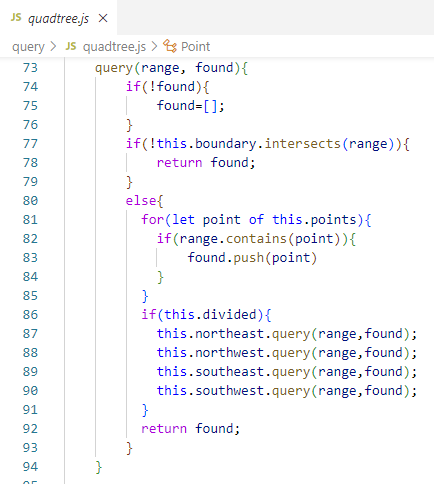
\includegraphics[width=0.5\textwidth]{Img/quadtree_query.png}
\caption{Algoritmo actualizado en el archivo quadtree.js}
\end{figure}

\begin{itemize}
   \item Editar el archivo sketch.js para hacer consultas con el mouse.
\end{itemize}

\begin{figure}[H]
\centering
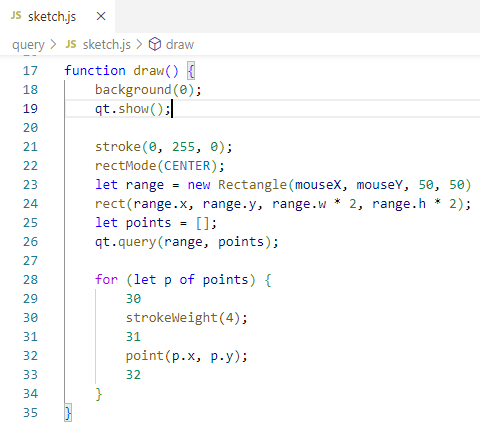
\includegraphics[width=0.65\textwidth]{Img/sketch_query.png}
\caption{Algoritmo actualizado en el archivo sketch.js}
\end{figure}

\begin{itemize}
   \item Resultado hasta el momento, se consultan puntos utilizando el mouse.
\end{itemize}

\begin{figure}[H]
\centering
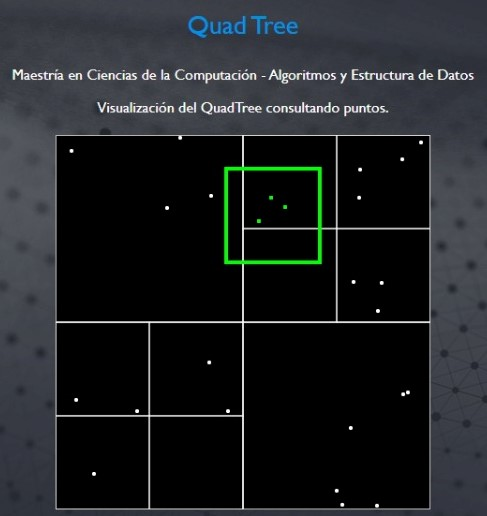
\includegraphics[width=0.5\textwidth]{Img/consultar_puntos_quadtree.jpeg}
\caption{Visualización Quadtree con consulta de puntos}
\end{figure}

    \item Estructura Octree

    \end{enumerate}

\section{Conclusiones}

\begin{itemize}
            \item 1
\end{itemize}
\begin{itemize}
            \item 2
\end{itemize}
	
	%\clearpage
	%\bibliographystyle{apalike}
	%\bibliographystyle{IEEEtranN}
	%\bibliography{bibliography}
		
	
\end{document}